\documentclass[12pt]{article}
\usepackage[margin=1in]{geometry} 
\usepackage{amsmath,amsthm,amssymb,amsfonts}
\usepackage{graphicx} 
\usepackage{tabularx} 


\begin{document}
 
 
\title{Analysis and Classification of Crimes in Chicago}
\author{Ye Zhou}
\maketitle
 
\section{Definition}
\subsection{Project Overview}
Historically, Chicago saw a major rise in violent crime starting in the later 1960s. More recently, the crime situation in Chicago is getting even worse. Last year, Chicago has experienced a recent spike in homicides of 762 people, an increase of 58 percent over 2015. Compared with other largest cities in United States, Chicago has a significantly higher murder rate than New York or Los Angeles. There is no denying the fact that crimes have become a severe social concern for Chicago as prosperous communities in the long term. 
\subsection{Problem Statement}
This project is aimed to analyze Chicago crimes in 2015 and 2016 and make prediction of crime category based on time and position information. The raw data from Chicago Data Portal is pre-processed to features (year, month, weekday, hour, location description, domestic, beat, district, ward, community area, latitude and longitude) and target variable (crime type). $20\%$ of the data is randomly sampled and then split into train and test data sets (6:4). After an exploration in the visualization of the crime data, the logistic regression (benchmark model) is applied as a Benchmark model.  At the end, a Xgboost model is trained on train data set and hype-parameters are tuned using k-fold cross-validation. The performance of two models are evaluated and compared in the means of log loss function and accuracy on the test data set.

\subsection{Metrics} 
This project use the log loss function and accuracy, from \verb|sklearn.metrics| package, to train models and evaluate the performance.

\section{Analysis}
\subsection{Data Exploration}
The data is imported from the Chicago Data Portal website [4], which is a collection of city data related not only to crimes, but also to education, transportation, health, and so on.
The data set has 21 columns:
\begin{itemize}
\item ID - Unique identifier for the record.
\item Case Number - The Chicago Police Department RD Number (Records Division Number), which is unique to the incident.
\item Date - Date when the incident occurred. this is sometimes a best estimate.
\item Block - The partially redacted address where the incident occurred, placing it on the same block as the actual address.
\item IUCR - The Illinois Unifrom Crime Reporting code. This is directly linked to the Primary Type and Description.
\item Primary Type - The primary description of the IUCR code. It is target variable to predict in the project. The distribution of crime types is shown in Figure \ref{fig:count}.
\item Description - The secondary description of the IUCR code, a subcategory of the primary description.
\item Location Description - Description of the location where the incident occurred.
\item Arrest - Indicates whether an arrest was made.
\item Domestic - Indicates whether the incident was domestic-related as defined by the Illinois Domestic Violence Act.
\item Beat - Indicates the beat where the incident occurred. A beat is the smallest police geographic area – each beat has a dedicated police beat car. Three to five beats make up a police sector, and three sectors make up a police district. The Chicago Police Department has 22 police districts.
\item District - Indicates the police district where the incident occurred.
\item Ward - The ward (City Council district) where the incident occurred.
\item Community Area - Indicates the community area where the incident occurred. Chicago has 77 community areas.
\item FBI Code - Indicates the crime classification as outlined in the FBIs National Incident-Based Reporting System (NIBRS).
\item X Coordinate - The x coordinate of the location where the incident occurred in State Plane Illinois East NAD 1983 projection. This location is shifted from the actual location for partial redaction but falls on the same block.
\item Y Coordinate - The y coordinate of the location where the incident occurred in State Plane Illinois East NAD 1983 projection. This location is shifted from the actual location for partial redaction but falls on the same block.
\item Year - Year the incident occurred.
\item Updated On - Date and time the record was last updated.
\item Latitude - The latitude of the location where the incident occurred. This location is shifted from the actual location for partial redaction but falls on the same block.
\item Longitude - The longitude of the location where the incident occurred. This location is shifted from the actual location for partial redaction but falls on the same block.
\item Location - The location where the incident occurred in a format that allows for creation of maps and other geographic operations on this data portal. This location is shifted from the actual location for partial redaction but falls on the same block.
\end{itemize}

\begin{figure}[ht]
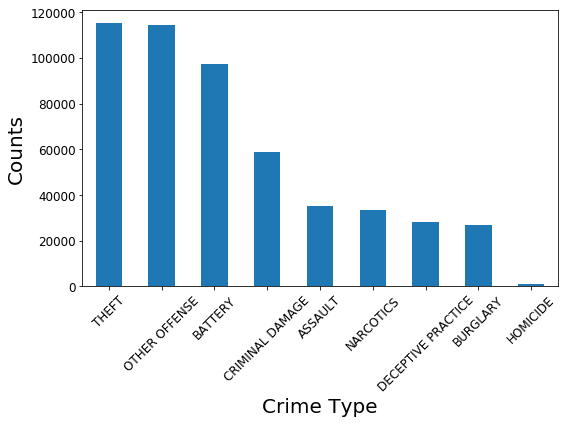
\includegraphics[scale=0.5]{figure/total_crime.png}
\centering
\caption{Total crimes in Chicago in 2015 and 2016}
\label{fig:count}
\end{figure}
  
\subsection{Exploratory Visualization}
The features related to time are 'Year', 'Month' and 'Hour', extracted from the original feature 'Date'. As shown in figure \ref{fig:time}a, in the past two years, Chicago experienced a high spike of crimes from May to October and has the lowest crime commits in February. Figure \ref{fig:time}b represents the data, relying on the principal component analysis, where the first principal component corresponds to the direction with the largest variation. The biplot represents the axes of crime types and data point on the first two principal components (PCs). The first PC shows consistently that there are generally more crimes from May to October. The second PC indicates that BATTERY and NARCOTICS have a higher frequency in May and June, while THEFT occurs more from September to October. The biplot of the crime counts by hour and crime types is shown in Figure \ref{fig:time}c. The first PC shows generally more crimes from noon to midnight. The second principal component shows that BATTERY and OTHER OFFENSE have a higher frequency at night (from 19 to 23), while THEFT and DECEPTIVE PRACTICE occurs more in the afternoon (from 12 to 15). Figure \ref{fig:time}d shows a comparison of crimes between 2015 and 2016 for different crime types. A more detailed table of crime annual increase rate are shown in Table \ref{tab:year}, which shows that the count of Homicide crime increases by $60.60\%$ from 2015 to 2016, while that of Narcotics is reduced by $53\%$.  

\begin{table}
\caption{Annual crime increase rate from 2015 to 2016 in Chicago} 
\label{tab:year} 
\begin{center}
\begin{tabular}{l|p{2.5cm}|p{2.5cm}|c}
\hline
\textbf{Primary Type}&	\textbf{2015}&	\textbf{2016}	&	\textbf{Increase rate}\\
\hline		
ASSAULT&			16945&	18076&	6.67\\
BATTERY&			48578&	48666&	0.18\\
BURGLARY&		13084&	13619&	4.09\\
CRIMINAL DAMAGE&	28527&	30185&	5.81\\
DECEPTIVE PRACTICE&	14577&	13507&	-7.34\\
HOMICIDE&		467&		750&		60.60\\
NARCOTICS&		22839&	10662&	-53.32\\
OTHER OFFENSE&	57744&	56690&	-1.83\\
THEFT&			56827&	58327&	2.64\\
\hline
\end{tabular}
\end{center}
\end{table}

The crime density on Chicago map is shown in Figure \ref{fig:pos}a, which shows that downtown area in Chicago has the highest crime density. Figure \ref{fig:pos}b shows the standardized crime count (divide by the maximum value among all communities) in each community for the past two years. The community shapefile is imported from the Chicago Data Portal website. Austin, Near North Side, Near West Side, South Shore are communities with standardized value greater than $0.5$. Position related features are Location Description, Domestic, Beat, District, Ward, Community Area, Latitude, Longitude. The crime counts in different location for different types are shown in Figure \ref{fig:location}a. The crime dependence on the Domestic feature is shown in Figure \ref{fig:location}c.  
Beat, District, Ward and Community Area are different ways of Chicago city district assignment. In this report, Community is used as an example for analysis. From Figure \ref{fig:location}b, the second PC shows that BATTERY and NARCOTICS have a higher frequency in AUSTIN, while THEFT occurs more near Chicago downtown (LOOP and NEAR NORTH SIDE). A more careful look at the district distribution of different crime types are shown in Figure \ref{fig:community}. It shows that Austin is the community with high crime rate of BATTERY, CRIMINAL DAMAGE, ASSAULT, NARCOTICS and OTHER OFFENSE; THEFT and DECEPTIVE PRACTICE occurred more near downtown; and BURGLARY has high outbreak in southern (e.g. South Shore) and western communities.

\begin{figure}[ht]
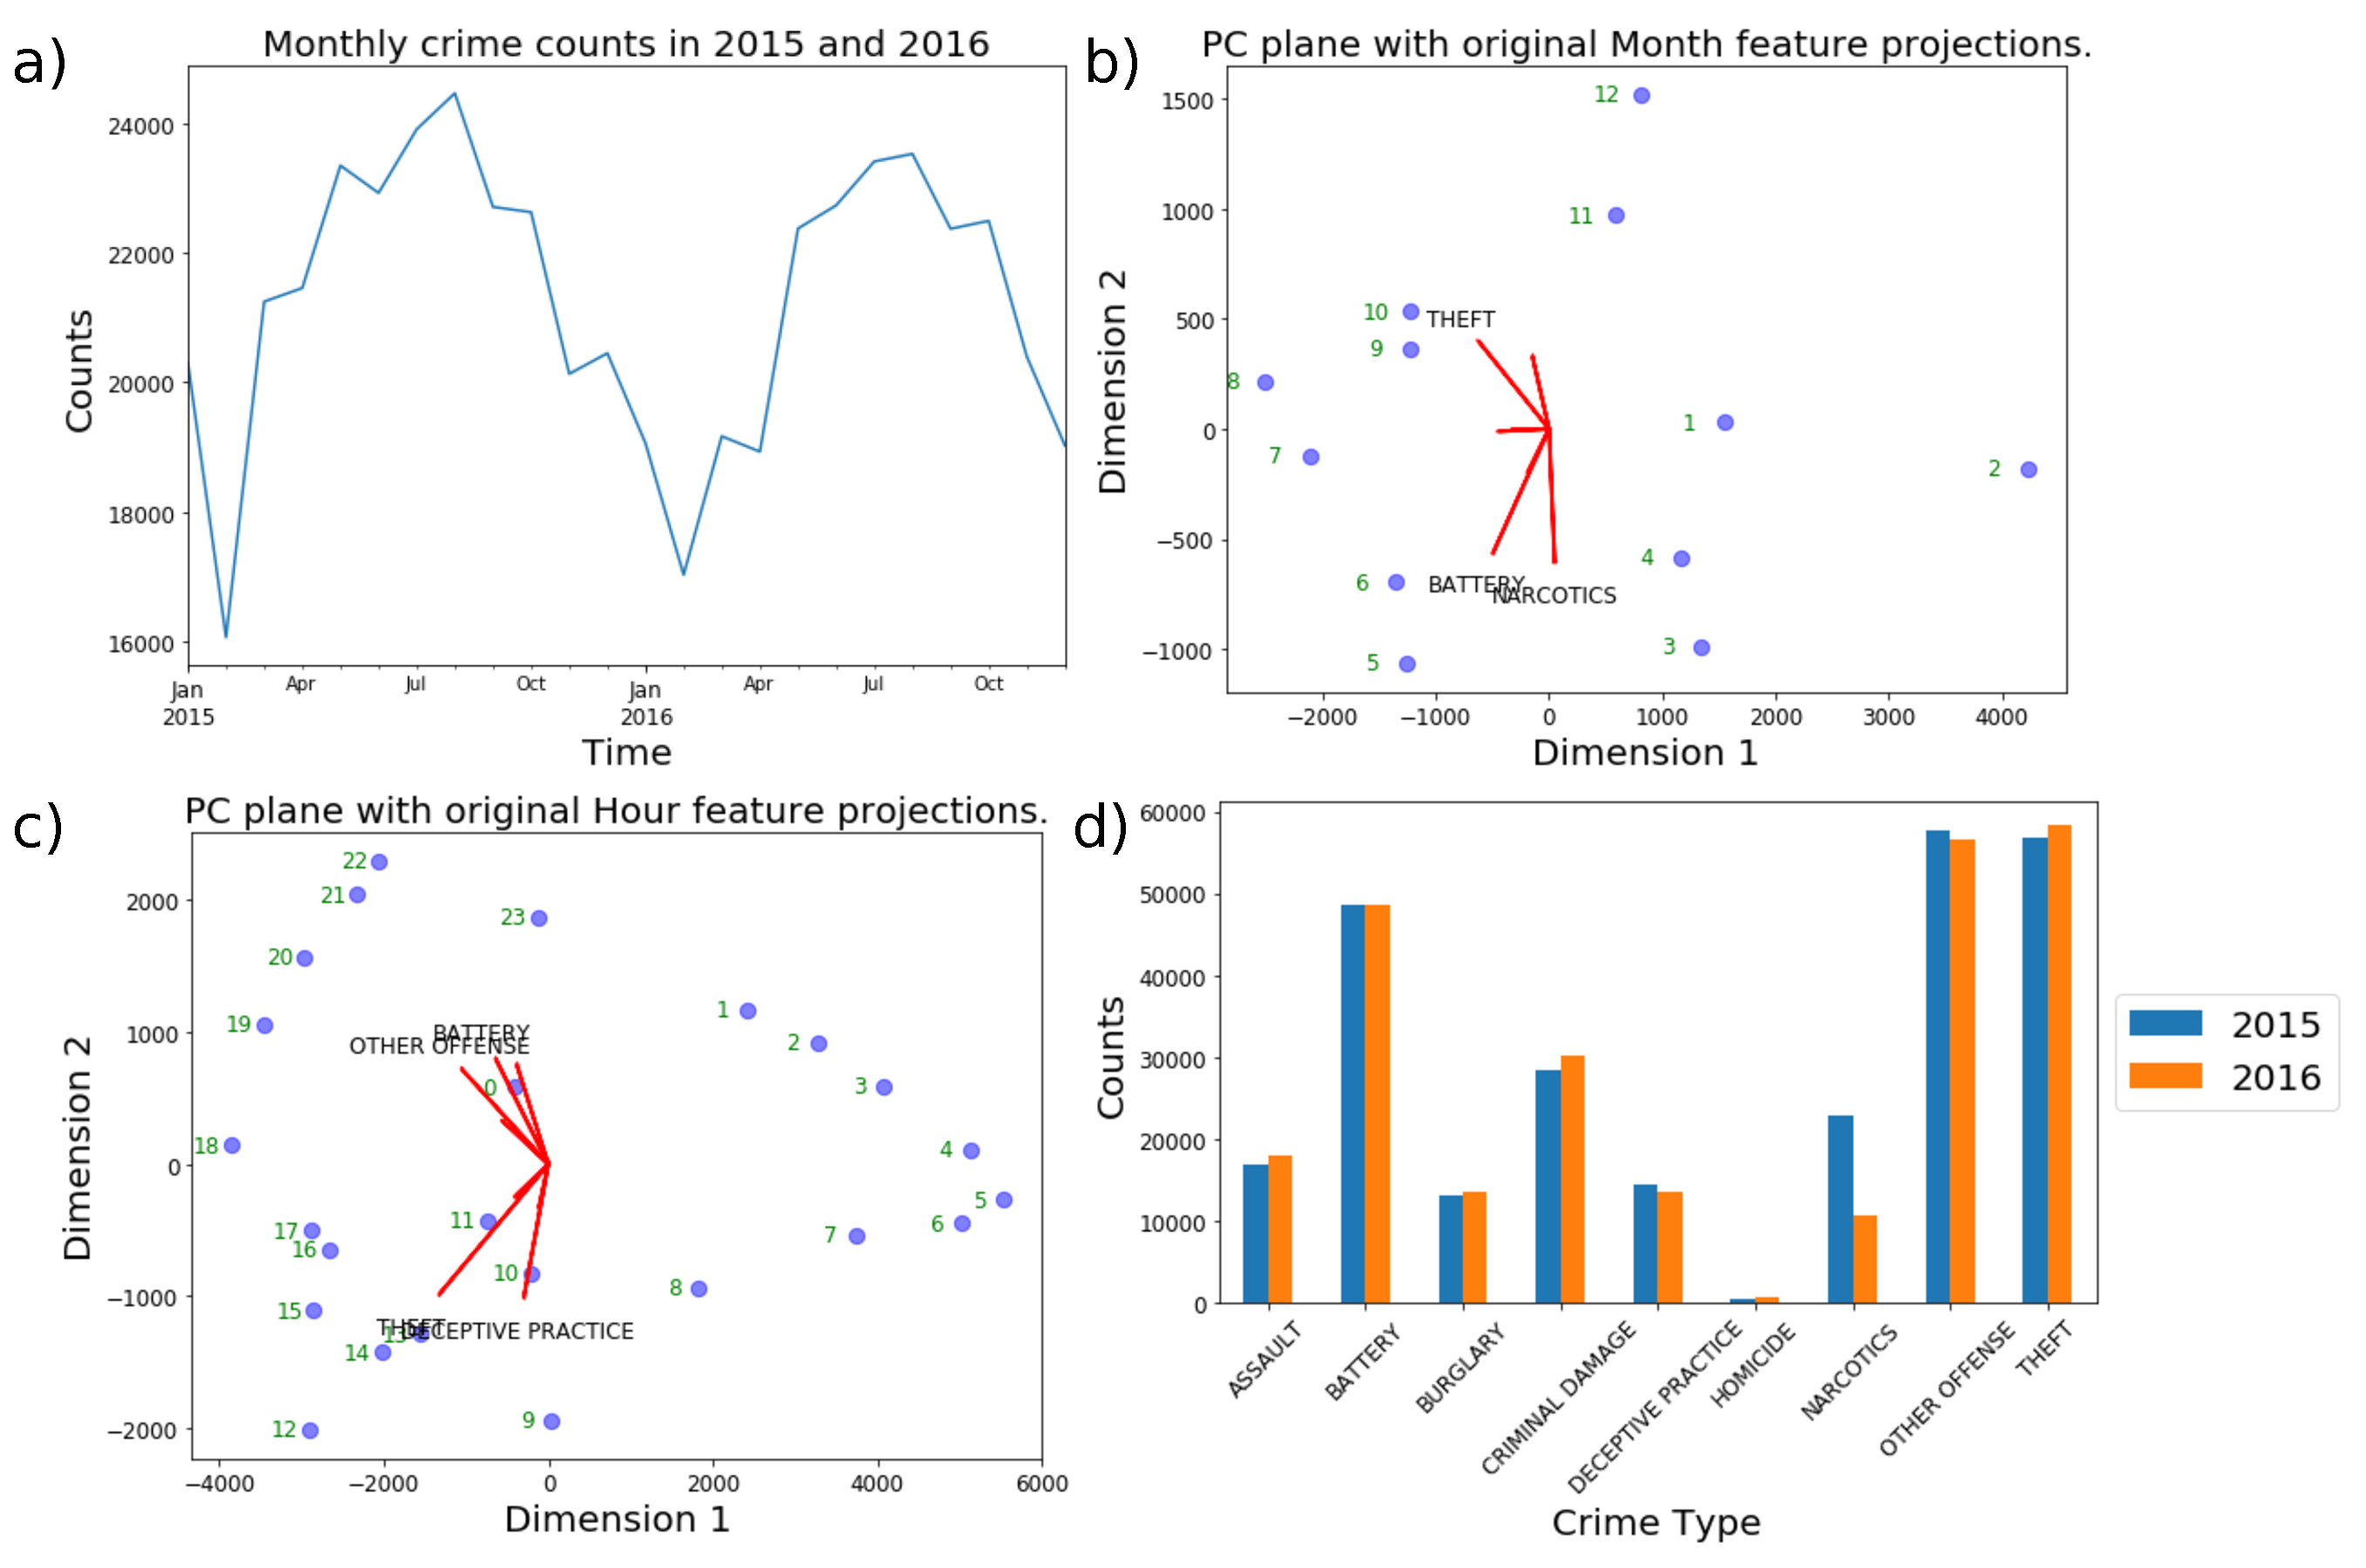
\includegraphics[scale=0.3]{figure/time.eps}
\centering
\caption{a) The monthly crime counts in Chicago from 2015 to 2016. b) Principal component analysis of crimes by month and type. c) Principal component analysis of crimes by hour and type. d) Comparison of crime count between 2015 and 2016.}
\label{fig:time}
\end{figure}

\begin{figure}[ht]
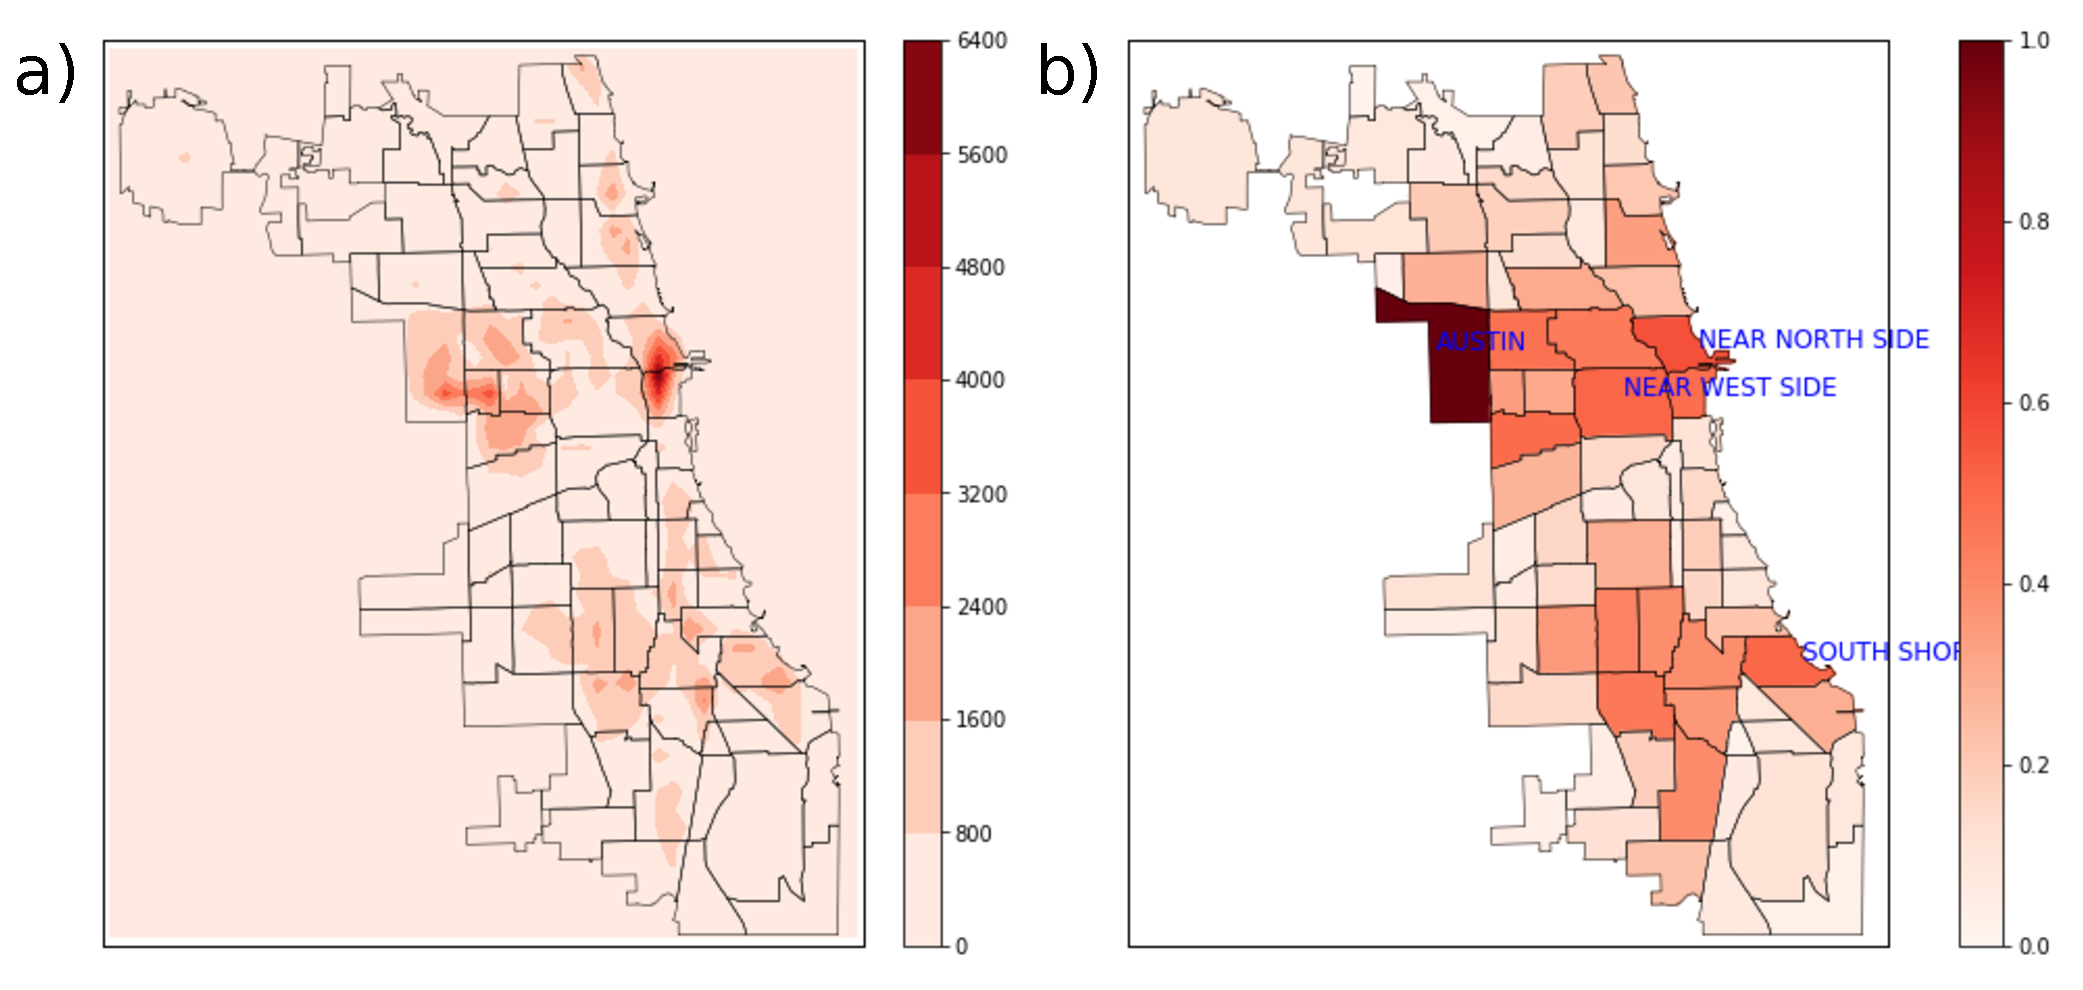
\includegraphics[scale=0.4]{figure/pos.eps}
\centering
\caption{a) Crime density in Chicago in 2015 and 2016. b) Crimes in Chicago communities.}
\label{fig:pos}
\end{figure}


\begin{figure}[ht]
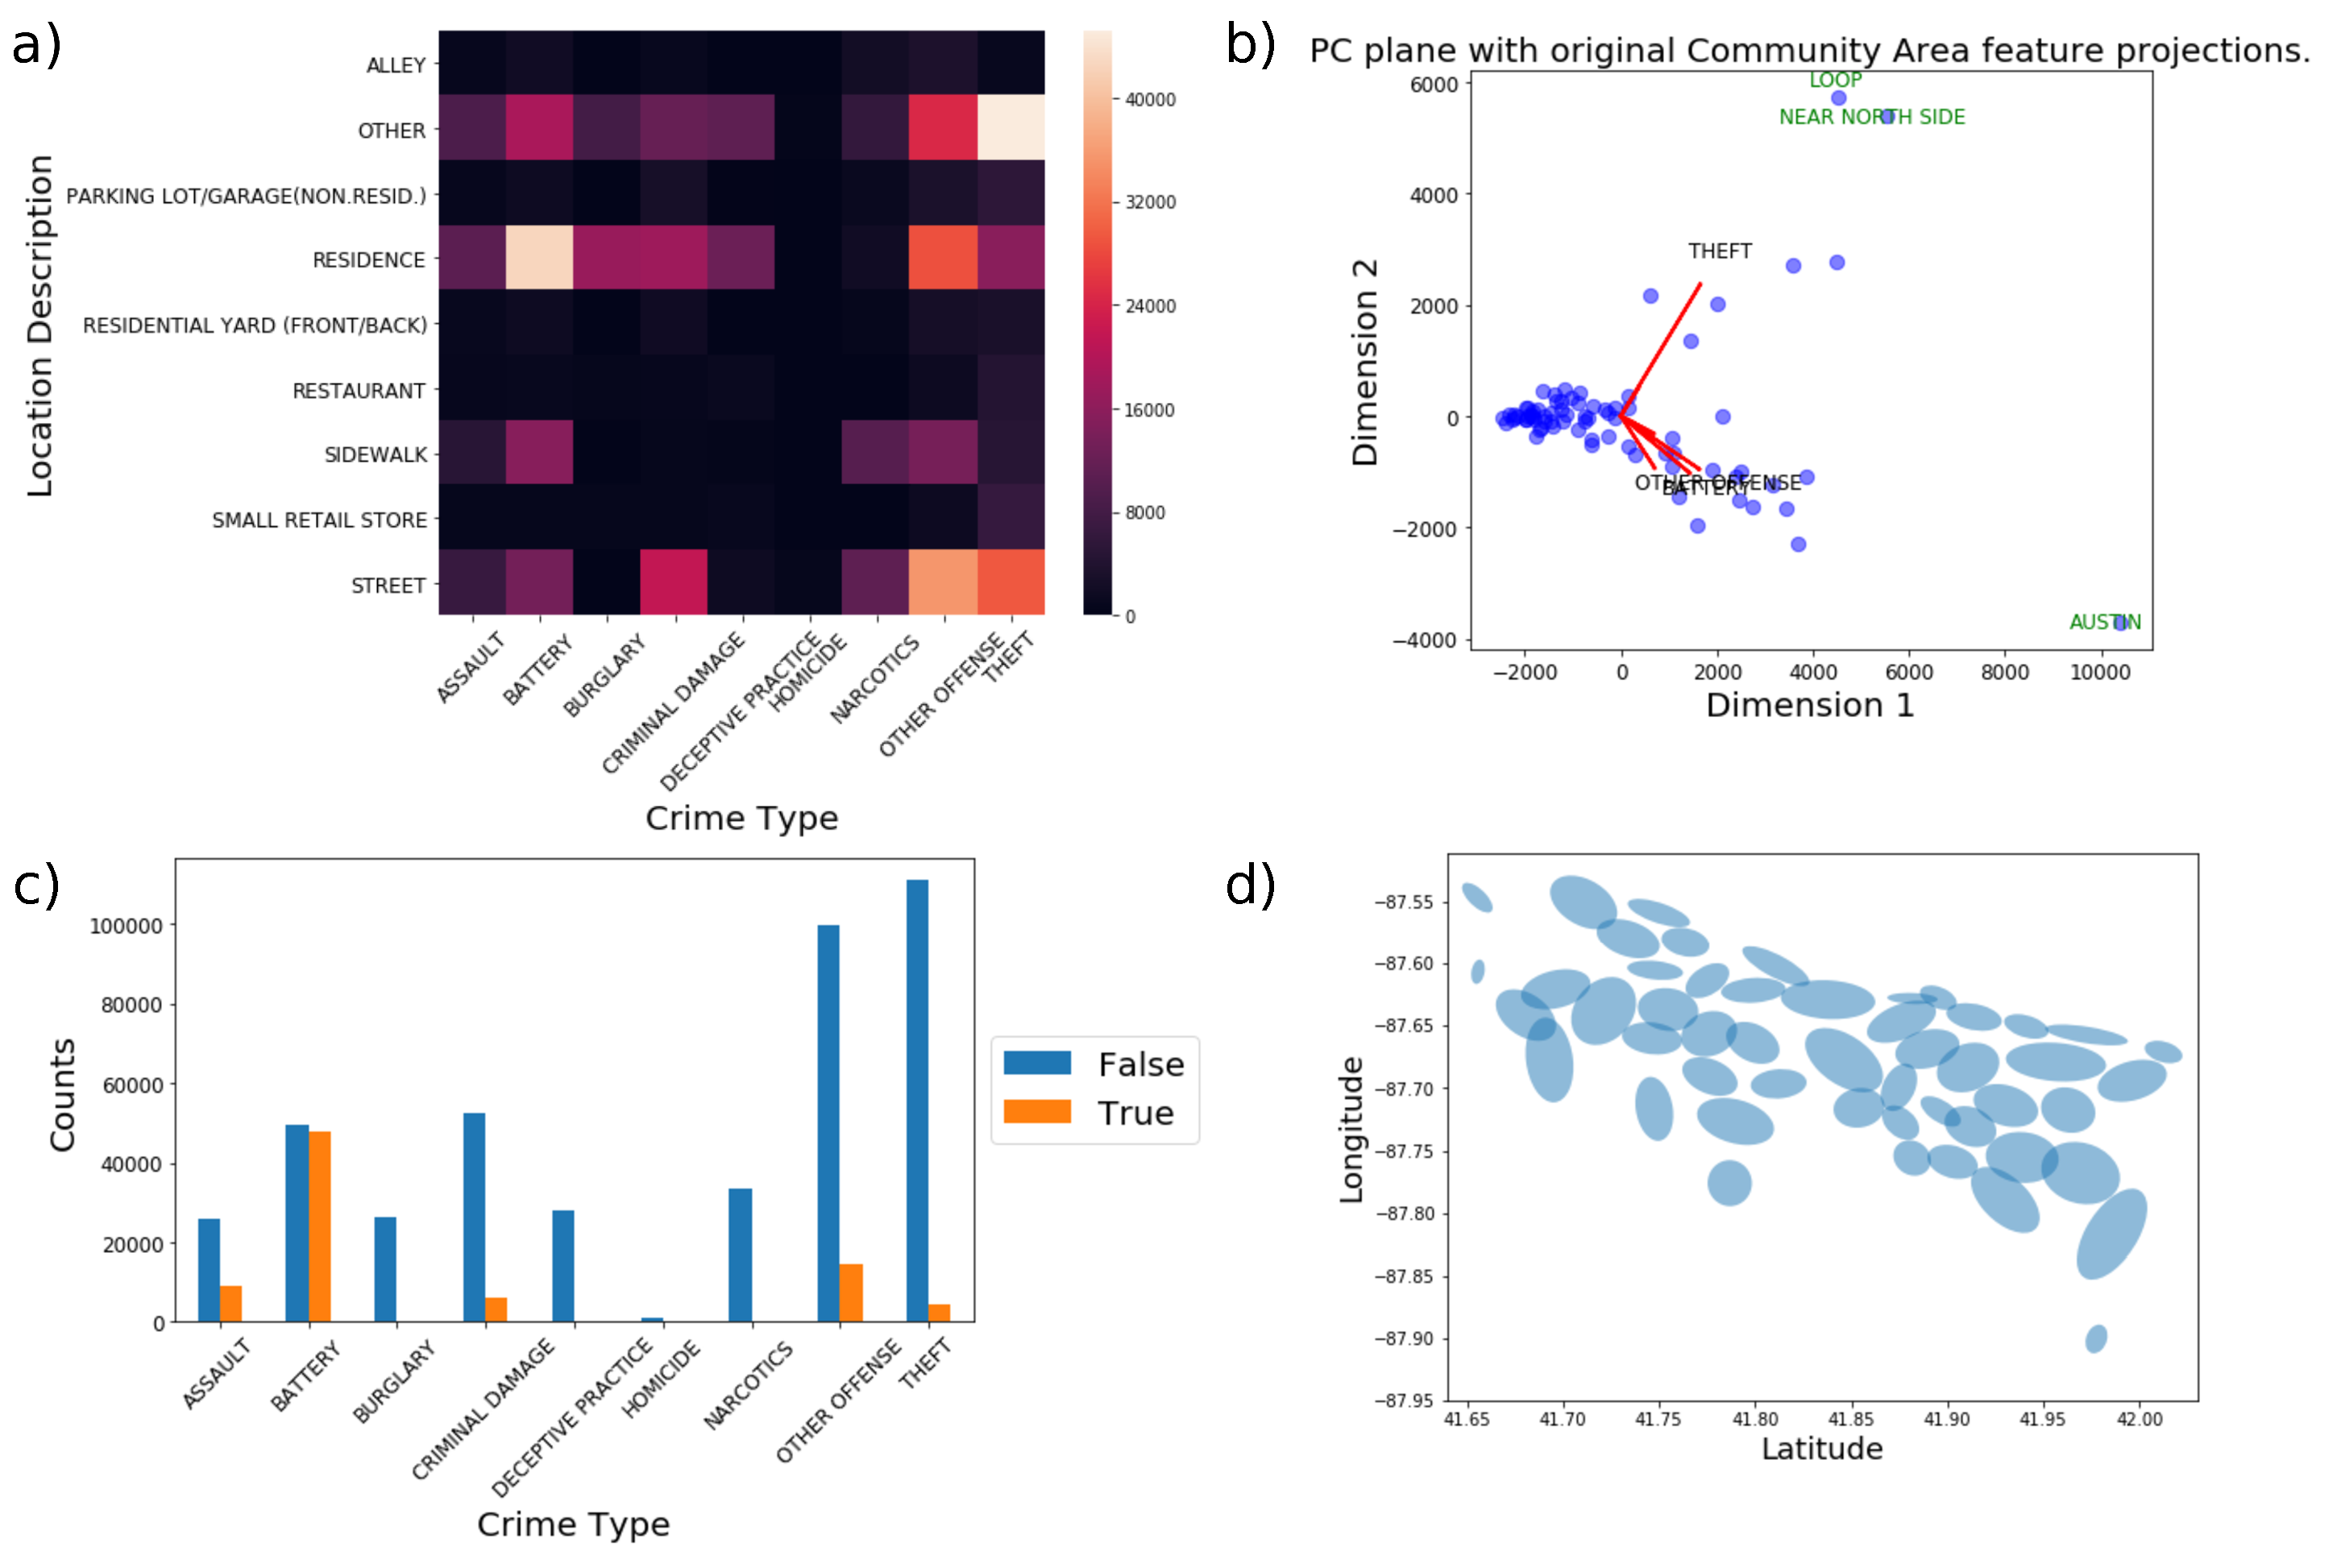
\includegraphics[scale=0.3]{figure/location.eps}
\centering
\caption{a) Relation between location description and crime type. b) Principal component analysis of crimes by community and type. c) Domestic related and unrelated crimes for different crime types in Chicago. d) Clusters of crimes by latitude and longitude using Gaussian Mixture Model.}
\label{fig:location}
\end{figure}

\begin{figure}[ht]
\includegraphics[scale=0.35]{figure/community.eps}
\centering
\caption{Standardized crime count in Chicago communities from 2015 to 2016 for different crime types.}
\label{fig:community}
\end{figure}

\subsection{Algorithms and Techniques}
In this project, the tree-based Gradient Boosting will be used with the package \verb|xgboost|, which is the abbreviation of 'extreme gradient boost'. This algorithm combines weak learners into one strong powerful learner. The hyper-parameters wait to be tuned are:

\begin{itemize}
\item \verb|learning_rate|: Boosting learning rate.
\item \verb|n_estimator|: number of boosted trees to fit.
\item \verb|min_child_weight|, which defines the minimum sum of weights of all observations required in a chiral.
\item \verb|max_depth|: the maximum depth of each weaker learner. Deep trees lead to over-fitting more easily.
\item \verb|gamma|: the minimum loss reduction required to make a split. Higher value prevents the model from over-fitting.
\item \verb|subsample|: the fraction of observations to be randomly samples for each tree. Lower value prevents the algorithm from over-fitting.
\end{itemize}


\subsection{Benchmark Model}
As a classification problem, the logistic regression model is used as a benchmark model. Logistic regression is a linear model, which could be used for the multi-class categorization. Two different regularization method, Ridge and Lasso will be tested with a range of regularization parameter values.
\begin{itemize}
\item \verb|penalty|: the norm used in the penalization.
\item \verb|C|: inverse of regularization strength .
\end{itemize}

\section{Methodology}
\subsection{Data Preprocessing}
The rows with NA values are dropped. New features, Month, Weekday (from Monday to Sunday) and Hour are created from original feature ‘Date’. The information of ‘IUCR’ and ‘FBI Code’ are excluded, because they contain the crime classification information. Despite the original positional features, new feature named 'Cluster' is created by clustering the latitude and longitude columns, using Gaussian Mixture Algorithm. 
The ‘Primary Type’ of crimes is the target variable for prediction, which has 33 categories in the 2016 crime data. To make the model more robust and efficient, the ‘Primary Type’ is transformed to major crime types (theft, battery, criminal damage, assault, deceptive practice, burglary, narcotics, robbery), and severe crime type (homicide). Figure \ref{fig:count} shows the total count of different crimes in Chicago from 2015 to 2016.

\subsection{Implementation}
\begin{itemize}
\item{\bf Data analysis} 
	\begin{itemize}
	\item \verb|Pandas|
	\item \verb|Numpy|
	\end{itemize}
\item{\bf Data visualization} 
	\begin{itemize}
	\item \verb|Matplotlib|
	\item \verb|seaborn|
	\item \verb|mpl_toolkits.basemap|
	\end{itemize}
\item{\bf Machine learning algorithms} 
	\begin{itemize}
	\item Principal component analysis: \verb|sklearn.decomposition.PCA|
	\item 'Location Description': \verb|sklearn.preprocessing.LabelEncoder|
	\item Clustering of Latitude and Longitude: \verb|sklearn.mixture.GaussianMixture |
	\item Data split: \verb|sklearn.model_selection.train_test_split|
	\item Logistic regression model: \verb|sklearn.linear_model.LogisticRegression|
	\item Xgboost model: \verb|xgboost|
	\item Metrics: \verb|sklearn.metrics.accuracy_score, log_loss|
	\end{itemize}
\end{itemize}

\subsection{Refinement}
Hyper parameter is tuned using \verb|sklearn.model_selection.GridSearchCV, KFold|.

\section{Results}
\subsection{Model Evaluation}
Two hyper-parameters, \verb|penalty| and \verb|C|, are tuned in the logistic regression, where \verb|penalty| denotes the type of regularization (Ridge or Lasso) and \verb|C| controls the regularization strength. The best parameters are chosen as ridge regression with \verb|C = 0.1| and final evaluation performance (log-loss function and accuracy) on the test data-set are 1.667 and $35.8\%$.
For the xgboost model, the hyperparameters corresponding to the best model is (grid search result saved in log files): 
\begin{itemize}
\item \verb|learning_rate = 0.1|
\item \verb|max_depth = 4|
\item \verb|gamma = 1|
\item \verb|n_estimators = 650|
\item \verb|subsample = 1|
\end{itemize}
The model performance (log-loss function and accuracy) on the test data set are 1.431 and $44.5\%$.

\subsection{Justification}
Compared with the accuracy of benchmark model ($35.8\%$), Xgboost algorithm obtained an enhanced accuracy rate near $44.5\%$. The final accuracy is four times better than the accuracy of random guess with 9-category output ($11.1\%$). 

\begin{figure}[ht]
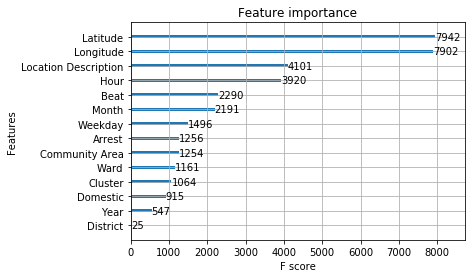
\includegraphics[scale=0.8]{figure/feature_importance.png}
\centering
\caption{Feature importance in the xgboost model for Chicago crime categorization problem.}
\label{fig:xgboost}
\end{figure}

\section{Conclusion}
\subsection{Free Form Visualization}
The analysis of feature importance from the Xgboost algorithm is shown in Figure \ref{fig:xgboost}. For the positional information, latitude and longitude are the most important features. The artificial feature, Cluster, created from these two features also plays certain role. Among all time dependent features, hour is the most related to the crime type in the model. 
\subsection{Reflection}
To sum up, this project is aimed to predict the Chicago crime type based on time and position information. The raw data from Chicago Data Portal is pre-processed to new features and target variable, and then split into train, test data set. After the exploration in the visualization of the crime data, we trained the logistic regression (benchmark model) and Xgboost models to obtain finely tuned parameters using k-fold cross-validation on training data set. The performance of two algorithms is evaluated with log loss function and accuracy and finally reported on the test data set. With Xgboost algorithm, the optimal accuracy rate is obtained at $44.5\%$, much better than the accuracy of random guess with 9-category output ($11.1\%$). 
\subsection{Improvement}
\begin{itemize}
\item Increase the data set. For instance, earlier crimes data might be included.
\item Feature engineering. In this project, 'Cluster' feature is created from the latitude and longitude features, which shows in certain feature importance in the Xgboost model. The import of new features, such as a binary feature holiday, may further improve the model performance.
\item Parameter tuning. Further examination of hyperparameters in the Xgboost model or cluster number in the Gaussian Mixture model may further enhance the model performance. 
\item Model selection. Other classifiers, such as Random Forest, K Nearest Neighbors, SVM, Neural Network, may be tested. 
\item Ensemble modeling. The results of different models may be synthesized to improve the accuracy of prediction.
\end{itemize}
\end{document}
